% ============================================================
%  Příprava na maturitu – Elektrotechnika
%  Okruh 5: Elektrické přístroje
% ============================================================

\documentclass[a4paper,10pt]{article}

\usepackage[T1]{fontenc}
\usepackage[utf8]{inputenc}
\usepackage[left=2.0cm, right=1.8cm, top=1.8cm, bottom=1.8cm]{geometry}
\usepackage{parskip}
\usepackage{xcolor}
\usepackage{tabularx}
\usepackage{booktabs}
\usepackage{tikz}
\usepackage{mdframed}
\usepackage{amsmath}
\usepackage{enumitem}
\usepackage{circuitikz}

\usetikzlibrary{arrows.meta, positioning, decorations.pathmorphing, shapes.geometric, calc}

% --- Barvy ---
\definecolor{accent}{HTML}{1A3A5C}
\definecolor{lightblue}{HTML}{EAF2F8}
\definecolor{lightyellow}{HTML}{FDFBE4}
\definecolor{lightgreen}{HTML}{EAF7EA}
\definecolor{lightred}{HTML}{FDE8E8}
\definecolor{lightgray}{HTML}{F4F4F4}

% --- Boxy ---
\newmdenv[backgroundcolor=lightblue,linecolor=accent!40,roundcorner=4pt,
  innertopmargin=6pt,innerbottommargin=6pt,innerleftmargin=8pt,innerrightmargin=8pt]{pojmybox}
\newmdenv[backgroundcolor=lightyellow,linecolor=accent!30,roundcorner=4pt,
  innertopmargin=6pt,innerbottommargin=6pt,innerleftmargin=8pt,innerrightmargin=8pt]{vysvetlenibox}
\newmdenv[backgroundcolor=lightgreen,linecolor=accent!40,roundcorner=4pt,
  innertopmargin=6pt,innerbottommargin=6pt,innerleftmargin=8pt,innerrightmargin=8pt]{vzorcebox}
\newmdenv[backgroundcolor=lightred,linecolor=accent!30,roundcorner=4pt,
  innertopmargin=6pt,innerbottommargin=6pt,innerleftmargin=8pt,innerrightmargin=8pt]{durazbox}

\setlist[itemize]{noitemsep, leftmargin=1.4em, topsep=2pt}
\setlist[enumerate]{noitemsep, leftmargin=1.4em, topsep=2pt}

% --- Zkratka pro jednotky ---
\newcommand{\jednotka}[1]{\,[\mathrm{#1}]}

\begin{document}

% ============================================================
\section*{\large Okruh 5 – Elektrické přístroje}

\begin{pojmybox}
\textbf{Klíčové pojmy:}
elektrický přístroj, spínání, vypínač, odpojovač, pojistka, jistič (MCB), bimetal, zkratová spoušť, proudový chránič (RCD), reziduální proud, stykač, relé, elektrický oblouk
\end{pojmybox}

\begin{vysvetlenibox}

% ================================================================
\subsection*{1. Rozdělení elektrických přístrojů}

Elektrické přístroje jsou zařízení, která slouží k ovládání, jištění, ochraně, měření nebo regulaci elektrických obvodů. Dělíme je primárně podle funkce:
\begin{itemize}
  \item \textbf{Spínací:} vypínače, přepínače, stykače, relé.
  \item \textbf{Jistící:} pojistky, jističe, nadproudová relé (chrání obvod).
  \item \textbf{Ochranné:} proudové chrániče, svodiče přepětí (chrání osoby nebo zařízení před nebezpečnými stavy).
\end{itemize}

% ================================================================
\subsection*{2. Elektrický oblouk a jeho zhášení}

Při rozpojování kontaktů pod zátěží vzniká mezi oddalujícími se kontakty plazma – \textbf{elektrický oblouk}. Ten je silně vodivý a dosahuje teplot i přes $5000\,^\circ\mathrm{C}$, čímž opaluje kontakty.

\begin{durazbox}
\textbf{AC vs. DC zhášení oblouku} (\textit{Souvisí s Okruhem 4: Střídavý proud})\\
Střídavý proud (AC) přirozeně prochází nulou (100x za vteřinu v 50Hz síti). V tomto okamžiku oblouk na zlomek milisekundy zhasne a úkolem přístroje je zabránit jeho znovuzapálení (např. oddálením kontaktů nebo ochlazením). Stejnosměrný proud (DC) nulou neprochází, proto je zhášení DC oblouku mnohem náročnější a přístroje pro DC sítě musí být speciálně dimenzovány (např. magnetické vyfukování oblouku).
\end{durazbox}

% ================================================================
\subsection*{3. Jistící přístroje – Pojistky}

Slouží k ochraně obvodu před \textbf{zkratem} a extrémním \textbf{přetížením}.
\textbf{Princip:} Uvnitř keramického tělesa (vyplněného křemičitým pískem pro chlazení a zhášení oblouku) je tavný drátek. Průchodem nadproudu se drátek zahřeje a přetaví (přeruší obvod). Jedná se o jednorázový přístroj.

% ================================================================
\subsection*{4. Jistící přístroje – Jističe (MCB - Miniature Circuit Breaker)}

Jistič je samočinný vypínač, který při nadproudu rozpojí obvod. Lze jej znovu nahodit. Jistí proti dvěma stavům pomocí dvou spouští:

\begin{enumerate}
  \item \textbf{Tepelná spoušť (bimetal):} Reaguje na \textbf{přetížení} (mírné překročení jmenovitého proudu). Průchodem proudu se ohřívá pásek ze dvou kovů o různé teplotní roztažnosti. Pásek se ohne a mechanicky vybaví zámek. Reakce je pomalá (minuty).
  \item \textbf{Elektromagnetická (zkratová) spoušť:} Reaguje na \textbf{zkrat} (obrovský proud). Využívá Ampérovu sílu cívky (\textit{viz Okruh 3: Magnetické pole}). Kotva vtáhnutá magnetickým polem okamžitě rozpojí kontakty (reakce v řádech milisekund).
\end{enumerate}

\begin{center}
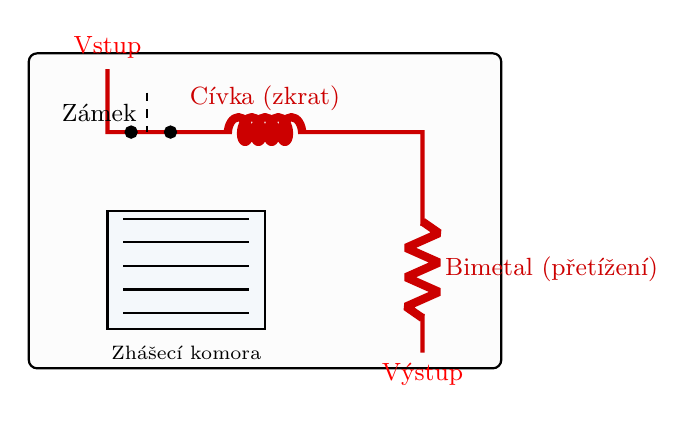
\begin{tikzpicture}[>=Stealth, font=\small, thick]
  % Tělo jističe
  \draw[fill=lightgray!30, rounded corners=3pt] (0,0) rectangle (6,4);
  
  % Proudová cesta
  \draw[red!80!black, line width=1.5pt] (1,3.8) -- (1,3) -- (2,3) 
    to[L, l=Cívka (zkrat)] (4,3) -- (5,3) -- (5,2) 
    to[R, l=Bimetal (přetížení)] (5,0.5) -- (5,0.2);
    
  % Kontakty
  \draw[fill=black] (1.3,3) circle (2pt);
  \draw[fill=black] (1.8,3) circle (2pt);
  \draw[dashed] (1.5, 3.5) -- (1.5, 3) node[midway, left] {Zámek};
  
  % Zhášecí komora
  \draw[fill=lightblue!50] (1,0.5) rectangle (3,2);
  \foreach \y in {0.7, 1.0, 1.3, 1.6, 1.9} \draw (1.2,\y) -- (2.8,\y);
  \node[font=\scriptsize] at (2,0.2) {Zhášecí komora};
  
  \node[above, red] at (1,3.8) {Vstup};
  \node[below, red] at (5,0.2) {Výstup};
\end{tikzpicture}
\end{center}

\textbf{Vypínací charakteristiky:}
\begin{itemize}
  \item \textbf{B} – pro spotřebiče bez rázů (žárovky, topení, běžné zásuvky). Zkratová spoušť reaguje při $3-5\times I_n$.
  \item \textbf{C} – pro stroje s rozběhovým proudem (motory, transformátory). Reakce při $5-10\times I_n$.
  \item \textbf{D} – pro obvody s obrovským rázovým proudem (svářečky). Reakce při $10-20\times I_n$.
\end{itemize}

% ================================================================
\subsection*{5. Proudové chrániče (RCD - Residual Current Device)}

Zatímco jistič chrání stroje a vedení, proudový chránič \textbf{chrání životy osob a zvířat} a zabraňuje vzniku požáru.

\textbf{Princip (Součtový transformátor proudu):} Využívá Faradayův zákon elektromagnetické indukce (\textit{viz Okruh 3}). Všechny pracovní vodiče (L i N) procházejí toroidním jádrem. 
Pokud je obvod v pořádku, proud tam ($I_L$) i zpět ($I_N$) je stejný, jejich magnetická pole se v jádře vyruší ($\Sigma I = 0$) a do sekundární cívky se neindukuje žádné napětí.
Pokud se člověk dotkne fáze a část proudu $I_\Delta$ odejde do země, vznikne asymetrie ($I_L \neq I_N$). V jádře vznikne magnetický tok, který v sekundární cívce indukuje napětí a to okamžitě vybaví citlivé relé, které obvod rozpojí.

\begin{center}
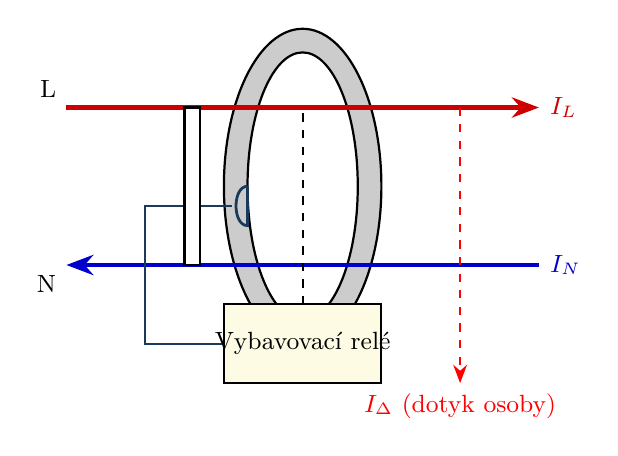
\begin{tikzpicture}[>=Stealth, font=\small, thick]
  % Toroidní jádro
  \draw[fill=gray!40, even odd rule] (3,1.5) ellipse (1 and 2) (3,1.5) ellipse (0.7 and 1.7);
  
  % Vodič L
  \draw[red!80!black, line width=1.5pt, ->] (0,2.5) -- (6,2.5) node[right] {$I_L$};
  \node[above left] at (0,2.5) {L};
  
  % Vodič N
  \draw[blue!80!black, line width=1.5pt, <-] (0,0.5) -- (6,0.5) node[right] {$I_N$};
  \node[below left] at (0,0.5) {N};
  
  % Unikající proud (do země)
  \draw[dashed, red, ->] (5,2.5) -- (5, -1) node[below] {$I_\Delta$ (dotyk osoby)};
  
  % Sekundární vinutí
  \draw[accent, line width=1pt] (2.3,1.5) to[out=180,in=180] (2.3, 1) -- (2.3, 1.5); % Zjednodušená cívka
  \draw[accent] (2.1, 1.25) -- (1, 1.25) -- (1, -0.5) -- (2, -0.5);
  \draw[fill=lightyellow] (2,-1) rectangle (4,0);
  \node at (3,-0.5) {Vybavovací relé};
  
  % Propojení relé na kontakty
  \draw[dashed] (3, 0) -- (3, 2.5);
  \draw[fill=white] (1.5, 2.5) rectangle (1.7, 0.5);
  
\end{tikzpicture}
\end{center}

\begin{vzorcebox}
\[
\Delta I = | I_L - I_N |
\]
Jmenovitý reziduální proud pro ochranu osob: $\Delta I_n = 30\,\mathrm{mA}$ (čas vypnutí $< 0{,}3\,\mathrm{s}$).
\end{vzorcebox}

% ================================================================
\subsection*{6. Stykače a Relé}

Jsou to spínací přístroje ovládané elektromagnetem (\textit{viz Okruh 3}). Umožňují \textbf{malým výkonem} (např. tlačítko, PLC automat, čidlo) \textbf{ovládat velké výkony} (motory, topná tělesa).

\begin{itemize}
  \item \textbf{Relé:} Malý přístroj pro spínání malých výkonů a řídicích signálů (pomocné kontakty).
  \item \textbf{Stykač:} Mohutný přístroj konstruovaný pro spínání velkých výkonů a motorů. Obsahuje silové (hlavní) kontakty vybavené zhášecími komorami a pomocné kontakty (pro signalizaci a samočinné přidržení).
\end{itemize}

\begin{center}
\begin{circuitikz}[font=\small]
  % Řídicí obvod (Cívka)
  \draw (0,2) to[short, o-] (1,2) to[normal open switch, l=Tlačítko START] (3,2) 
    to[cute inductor, l=Cívka (A1-A2)] (3,0) to[short, -o] (0,0);
  \node[left] at (0,2) {+24V (Ovládání)};
  \node[left] at (0,0) {0V};

  % Mechanická vazba
  \draw[dashed, gray, thick] (3.5, 1) -- (5.5, 1);

  % Silový obvod (Kontakty)
  \draw (6,2) to[short, o-] (7,2) to[normal open switch, l=Hlavní kontakty (L1)] (7,0) to[short, -o] (6,0);
  \node[left] at (6,2) {400V (Silovina)};
  \node[left] at (6,0) {K motoru};
\end{circuitikz}
\end{center}

\end{vysvetlenibox}

\end{document}